%sri
\documentclass[conference]{IEEEtran}
\IEEEoverridecommandlockouts
% The preceding line is only needed to identify funding in the first footnote. If that is unneeded, please comment it out.
\usepackage{cite}
\usepackage{amsmath,amssymb,amsfonts}
\usepackage{algorithmic}
\usepackage{graphicx}
\usepackage{textcomp}
\def\BibTeX{{\rm B\kern-.05em{\sc i\kern-.025em b}\kern-.08em
    T\kern-.1667em\lower.7ex\hbox{E}\kern-.125emX}}
\begin{document}

\title{As Much Resilience As You Want: \\Application-tailored Resilience in Legion}

%\author{\IEEEauthorblockN{Karthik Murthy} \and
%\IEEEauthorblockN{Mike Bauer} \and 
%\IEEEauthorblockN{Manolis Papadakis} \and
%\IEEEauthorblockN{Kyushick Lee} \and
%\IEEEauthorblockN{Yongkee Kwon} \and
%\IEEEauthorblockN{Wonchan Lee} \and
%\IEEEauthorblockN{Todd Warszawski} \and 
%\IEEEauthorblockN{Elliott Slaughter} \and
%\IEEEauthorblockN{Sean Treichler} \and
%\IEEEauthorblockN{Alex Aiken} \and
%\IEEEauthorblockN{Mattan Erez}
%}

\maketitle

\begin{abstract}
Resilient is an important aspect of scaling applications on
large clusters. As we approach parallelism profiles of several millions and long running applications, we need to ensure that ineffect ``we reach the end".
Defining the policy interaction with the programming model features necessitates that we revisit the memory concistency model. 
Recoverability, a critical step in
resilience, opens the door to optimizations such as speculation. We also
evaluate this.  \dots
\end{abstract}

\begin{IEEEkeywords}
resilience, legion
\end{IEEEkeywords}

\section{Introduction}

what is the need for resilience\\

what are the challenges we face with resilience in a deferred execution model, with all the decisions taken at runtime via a mapper ? \\

what are the advantages that we derive from the same ?\\
The needle in the resilience spectrum can be much finer than ABFT, sub-tree DAG based, snapshot based, relocatable-finish based, strategies. Dynamic and deferred being the key.

what are the advantages that we derive from having multiple wavefront ?\\
how do we ensure minimal overhead ?\\

Is it really a resilience framework, or a glorified garbage collector ?\\


how is it different from x10, parsec, charm++\\
	- they also allow tasks to be marked as resilience\\
	- x10 allows finish blocks, exception semantics.\\
	- what are the exception semantics that we are providing\\


what about regent ? where do we stand there ?\\

what about local vs global recovery\\
	- can we recover from a node failure\\
	- can we recover from an exception, what are the semantics that we provide here\\
	- can we recover from ECC errors, \\
	- can we fix these errors ?\\
	- can we recover from I/O errors ?\\ 
	- can we recover from non-SingleTasks, what is recovery for index space tasks, must epoch tasks\\

what is the memory consistency model ? what is the state of the regions, the tasks that are physically dependent but are not logically dependent ?\\
	

experiments: circuit, miniAero, Soleil-X, stencil, (S3D ?)\\

\begin{figure}
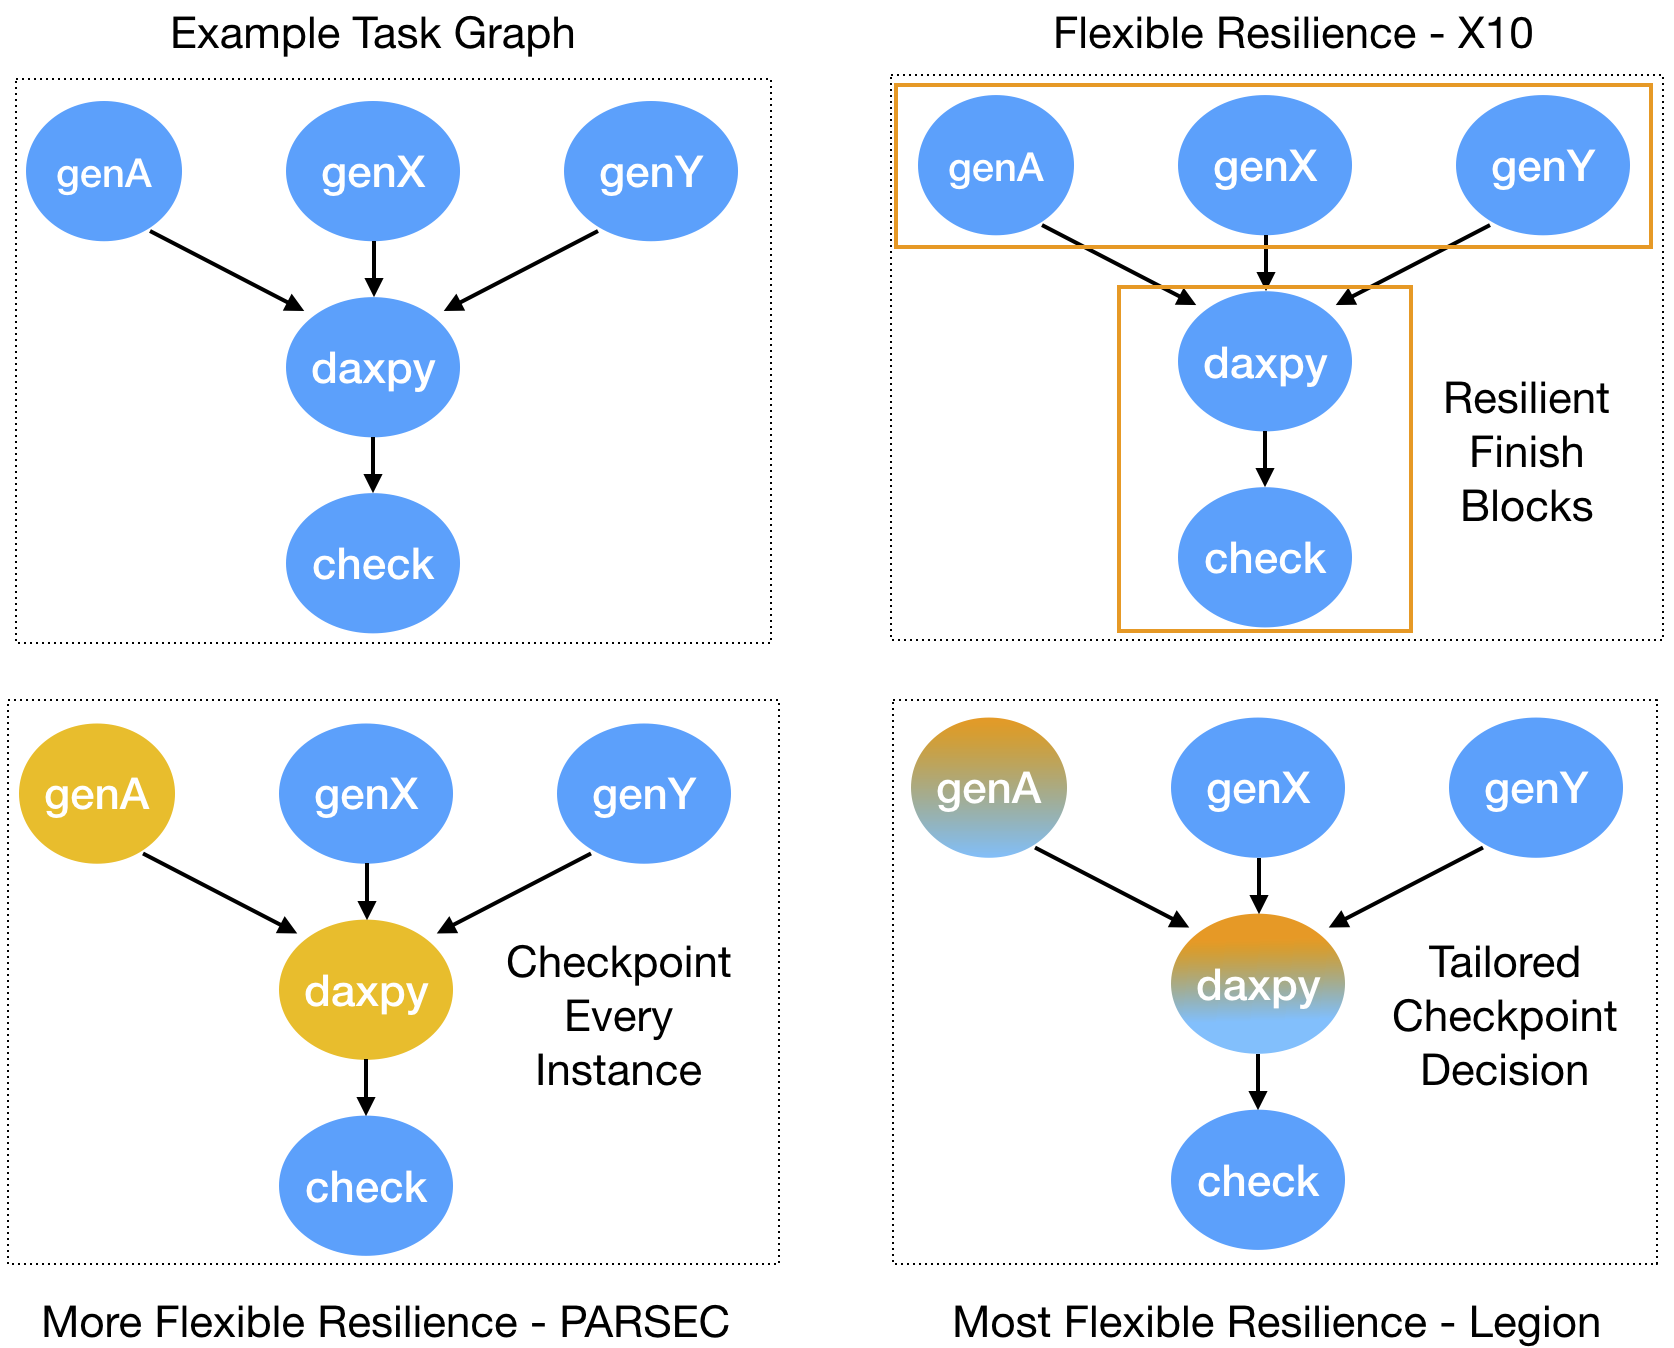
\includegraphics[width=.45\textwidth]{images/spectrum_x10_parsec_legion_policies.png}
\caption{A spectrum of resilience policies supported by different state-of-the-art parallel runtimes.}
\end{figure}


%sri

\section{Overview of Resilience in Legion}


%sri

\section{Interaction of Resilience Policy with Legion Features} 

which are the legion features of importance ?

put a figure of interaction.

what is the memory consistency angle here ?

what does it mean to advance the commit wavefront

Resilience is a tangling of the lifetime of a task and a region snapshot- 
1) when can we advance a commit wavefront ?
2) whats the lifetime of a region-instance snapshot ?

on this front, we see it as a two-step process a) define a consistent cut of tasks problem, b) commit any task strictly behind this wavefront c) garbage collect any snapshot that serves as input to any task that is already committed

consistent cut of tasks that can be part of the commit wavefront: 
a set of tasks whose inputs are need\_preserve'ed, or they are strictly post-dominated by tasks whose inputs are need\_preserved.  

3) what about copy/index/tasks ?
copy local to local follows the above semantics
copy local to remote get committed immediately after successful execution.
index launch tasks, actually feel need not be in the task graph, unless virtual mapping is used. they can be garbage collected immediately after all child tasks are included in the dependence analysis wavefront
  - I am thinking we will never have a case where are relaunching the index launch, since hte child tasks either are part of the committed wavefront or are not (pending a discussion on phase barriers)

Question on what to do about must\_epoch tasks with phase\_barrier inside them ?

answer: restartable phase\_barrier with generation commit callback 


\section{Implementation of Resilience}

\subsection{\texttt{need\_preserve} Implementation}

use current_versions inside legion_views.h TODO TODO

tagging region instances
tagging tasks

-the mapper marks an instance as persistent, i.e., vector<vector<bool>> persistent
-in finalize\_map\_task, the singleTask sees this and notes it down in the Individual\_task's persistent\_tasks list
-when trigger\_complete is called on the task, 

	1) inside line 5560, invalidate\_region\_tree\_contexts, 
		inside which we have runtime->forest->invalidate\_versions, we do not do on region[idx].region.
		we also do not do the instance\_top\_views
		
	2) we retain the mark on the task as allowed\_for\_gc.

   3) we go to the incoming of this task, and just like verified\_regions[true], we mark outgoing\_edge\_dominated[true]
      if all the outgoing of a task is marked as true, then we change allowed\_for\_gc = true.


Discussion Points for today
--------------------------
1) allow persistence on a subset of mapped instances in map\_task ? Pro:
flexibility, Con: if a checkpoint is to be considered useful for a restart, not
having the full set of inputs checkpointed seems contradictory. 
2) verify\_regions tracks op dependencies after physical dependence analysis, correct ? 
3) a discussion on persistence inside map\_task call 


discussed design:

1) build a function set\_hardened\_instnace(instance,task) along the lines of the set\_gc\_priority(instance, never, task) inside the mapper call
2) inside that mark a task's incoming edges as saying that it leads to a hardened instance(task)
3) the garbage collector will basically collect a task whose outgoing edges are all marked as verified/hardened.
4) if a task is gc'ed, then it marks all its incoming edges as leads to a hardened instance.
5) steps 1-4 will be based on set\_garbage\_collection\_priority and how verified\_regions are set. We will be adding a new list to each task, similar to verified\_regions, that will represent edges\_ending\_in\_hardened\_regions.


quash\_operation:
  847 line in realm/proc\_impl.cc tells us that we should set the poisoned to true and ensure that the start\_event.has\_triggered\_faultaware(poisoned) returns true

what about two sibling tasks that map the same instance, and one hardens it, the other does not
    - alex raised this, we discussed that trigger recover would check 
    - but the way we are doing it now, we are doing unverfied\_regions.erase based on even on guy below us who will call harden on a region instance
    - so the parent would have gone away, but the child B who did not call harden ont he physical region should be able to restart since the instance will be there
how to show thsi is working, if the application is too fast, then delete meta task on the logical region is called which deletes the region irrespective of whether its GC\_NEVER\_PRIORITY

REACTIVE
faulty task
   catch it
   poison propagation
   identify recovery point
   trigger\_recover

SEMANTICS
regions and instances and consistency

PROACTIVE
    mark instances as harden
    
DIFFERENCE WITH PARSEC:
    label a task with snapshot, i.e., all or none policy
    whereas we allow selective instances to be marked as harden.
      - what is an example app that is benefited by this ?

\subsubsection{Interaction of need\_preserve with the commit wavefront}
\subsubsection{Obtaining dependence graph in the mapper before calling need\_preserve} 


\subsection{ProfilingResponse callback used}
while using the profiling measurement reporting infrastructure as-is causes overhead, this is because of the invoking of a mapper profiling response function. We do not need that for resilience, so the resilience callback would short circuit it.

task launch -> porfiling reported event is there -> when it is triggered -> \texttt{singletask::profiling\_response} is invoked -> handle things
   ----- in here, there is no need to call the mapper side yet. So, avoid one overhead there, maybe this was never called and so , this is not an optimization. ok, back to square one. 

 


%sri


there are three different wavefronts in Legion, we can speculate on any of them. 


From a speculation perspective, are they different ? 
Are we novel, since we have these three different wavefronts ? 
Can we navigate through this, like the blanks 


1) execution wavefront 
what does it mean to speculate here, does the other steps have to be complete before we do this. 


2) mapping wavefront

3) dependence analysis wavefront


-- see mike's 6 wavefront answer.

There are three different wavefronts, there could

 
mike - speculation is more about tracking the resolution wavefront while resilience is more about tracking the commit wavefront, but the when things go bad, then i think the machinery to restart the mapping and execution wavefronts should be the same


%sri

\section{Experiments}

\subsection{Index Tasks}

\paragraph{Growth of memory as execution proceeds}
\paragraph{Performance overhead as execution proceeds}



\begin{center}
 \begin{tabular}{||c | c | c | c||} 
 \hline
 NumIter& No Resl No lg:res & No Res With lg:res & Res No lg:res \\ [0.25ex] 
 \hline\hline
100 &  7.2 & 6.6 & 23.6\\ 
 \hline
200 &  13.8 & 13.3 & 46.3\\ 
 \hline
400 &  26.1 & 26.5 & 94.4\\ 
 \hline
800 &  55 & 53 & 186.8\\ 
 \hline
1000 &  65 & 66 & 239.9\\ [1ex] 
 \hline
\end{tabular}
\end{center}

\begin{figure}
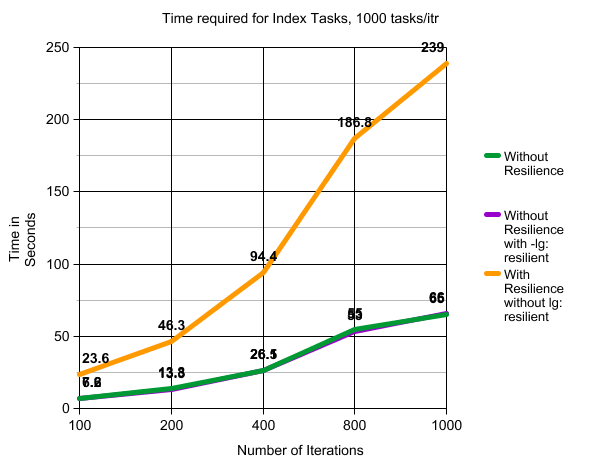
\includegraphics[width=\textwidth]{images/index_tasks_time.png}
\caption{Total time taken by 02\_index\_tasks. Time in Seconds, 1000 tasks/index launch }
\end{figure}


\begin{center}
 \begin{tabular}{||c | c | c | c||} 
 \hline
 NumIter& No Resl No lg:res & No Res With lg:res & Res No lg:res \\ [0.25ex] 
 \hline\hline
100 &  18 & 140 & 107 \\ 
 \hline
200 &  22 & 263 & 176 \\ 
 \hline
400 &  24 & 509 & 245 \\ 
 \hline
800 &  26 & 1002 & 428\\ 
 \hline
1000 & 26 & 1248 & 518\\ [1ex] 
 \hline
\end{tabular}
\end{center}

\begin{figure}
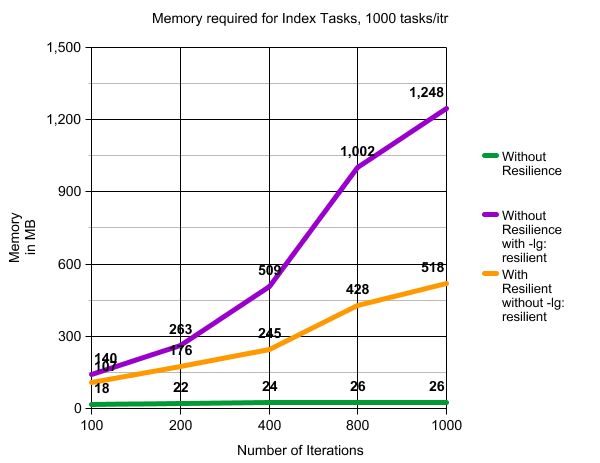
\includegraphics[width=\textwidth]{images/index_tasks_memory.png}
\caption{Total Memory footprint by 02\_index\_tasks. Memory in MB, 1000 tasks/index launch.}
\end{figure}





\subsection{Stencil}



\subsection{local recover vs global recovery}

\subsection{compute/comm vs no-failure/single failure/multi-failure}

\subsection{S3D, Pennant, Stencil, Circuit}

\subsection{Some Interesting Task Graphs for Recovery}





\section{Adaptive Resilience}
\section{Resilience Policy Implemented via Mapper: Example 1 Generic}
\section{Resilience Policy Implemented via Mapper: Example 2 UT Austin}


\input{related_work}

\section{Conclusion}

\section*{Acknowledgment}

\begin{thebibliography}{00}
\bibitem{b1} S. Treichler, M. Bauer, and A. Aiken. Language
support for dynamic, hierarchical data partitioning. In
Object Oriented Programming, Systems, Languages,
and Applications (OOPSLA), 2013.
\end{thebibliography}

\end{document}
